\documentclass{beamer}
%\documentclass[handout]{beamer}
% This file is a solution template for:

% - Giving a talk on some subject.
% - The talk is between 15min and 45min long.
% - Style is ornate.

% Copyright 2004 by Till Tantau <tantau@users.sourceforge.net>.
%
% In principle, this file can be redistributed and/or modified under
% the terms of the GNU Public License, version 2.
%
% However, this file is supposed to be a template to be modified
% for your own needs. For this reason, if you use this file as a
% template and not specifically distribute it as part of a another
% package/program, I grant the extra permission to freely copy and
% modify this file as you see fit and even to delete this copyright
% notice. 


\mode<presentation>
{
  \usetheme{Montpellier}

  %\setbeamercovered{transparent}
  % or whatever (possibly just delete it)
}

\usepackage{xcolor}
\usepackage{amsmath}

%\input ../macros.tex

\beamerdefaultoverlayspecification{<+->}

% Define a color for mathematical expressions
\definecolor{mathred}{RGB}{200,0,0}
\newcommand{\redmath}[1]{\textcolor{mathred}{#1}}

\usepackage[english]{babel}

\usepackage[latin1]{inputenc}
\usepackage{xcolor}
\usepackage{times}
\usepackage[T1]{fontenc}

% Or whatever. Note that the encoding and the font should match. If T1
% does not look nice, try deleting the line with the fontenc.

\title [Universal Portfolios] %(optional, use only with long paper titles)
{Universal Portfolios}

\author[Freund] % (optional, use only with lots of authors)
{Yoav Freund}
% - Give the names in the same order as the appear in the paper.
% - Use the \inst{?} command only if the authors have different
%   affiliation.

\institute[Universities of Somewhere and Elsewhere] % (optional, but mostly needed)

\subject{Machine Learning}
% This is only inserted into the PDF information catalog. Can be left
% out. 

% If you have a file called "university-logo-filename.xxx", where xxx
% is a graphic format that can be processed by latex or pdflatex,
% resp., then you can add a logo as follows:

% \pgfdeclareimage[height=0.5cm]{university-logo}{university-logo-filename}
% \logo{\pgfuseimage{university-logo}}



% Delete this, if you do not want the table of contents to pop up at
% the beginning of each subsection:
%% \AtBeginSubsection[]
%% {
%%   \begin{frame}<beamer>
%%     \frametitle{Outline}
%%     \tableofcontents[currentsection,currentsubsection]
%%   \end{frame}
%% }


% If you wish to uncover everything in a step-wise fashion, uncomment
% the following command: 

\beamerdefaultoverlayspecification{<+->}

\newcommand{\newmcommand}[2]{\newcommand{#1}{{\ifmmode {#2}\else\mbox{${#2}$}\fi}}}
\newcommand{\newmcommandi}[2]{\newcommand{#1}[1]{{\ifmmode {#2}\else\mbox{${#2}$}\fi}}}
\newcommand{\newmcommandii}[2]{\newcommand{#1}[2]{{\ifmmode {#2}\else\mbox{${#2}$}\fi}}}
\newcommand{\newmcommandiii}[2]{\newcommand{#1}[3]{{\ifmmode {#2}\else\mbox{${#2}$}\fi}}}

\newcommand{\algfnt}{\bf}

\newmcommand{\ouralg}{{\mbox{\algfnt Hedge}({\eta})}}

\newmcommand{\iter}{T}

\newfont{\cmmib}{cmmib10}
\newcommand{\boldell}{{\mbox{\cmmib \symbol{'140}}}}

\newmcommandi{\costvec}{{\boldell}^{#1}}
\newmcommandii{\cost}{{\ell}^{#1}_{#2}}

\newmcommandi{\rd}{\tilde{#1}}

\newmcommandi{\distvec}{{\bf p}^{#1}}
\newmcommandi{\rddistvec}{\rd{\bf p}^{#1}}
\newmcommandii{\dist}{{p}^{#1}_{#2}}
\newmcommandii{\rddist}{\rd{p}^{#1}_{#2}}

\newmcommandi{\bdistvec}{{\bf q}^{#1}}
\newmcommandii{\bdist}{{q}^{#1}_{#2}}

\newmcommandi{\wtvec}{{\bf w}^{#1}}
\newmcommandi{\rdwtvec}{\rd{\bf w}^{#1}}
\newmcommandii{\wt}{{w}^{#1}_{#2}}
\newmcommandii{\rdwt}{\rd{w}^{#1}_{#2}}

\newcommand{\w}[1]{\makebox[12pt]{{#1}}}
\newcommand{\Rps}{\mbox{\tt R}}
\newcommand{\rPs}{\mbox{\tt P}}
\newcommand{\rpS}{\mbox{\tt S}}
\newcommand{\rpstie}{\w{$\frac{1}{2}$}}
\newcommand{\rpswin}{\w{$0$}}
\newcommand{\rpsloss}{\w{$1$}}

\newmcommand{\decspace}{\Delta}
\newmcommand{\decsym}{\delta}
\newmcommandi{\dec}{\decsym^{#1}}
\newmcommand{\decdistsym}{\cal D}
\newmcommandi{\decdist}{{\decdistsym}^{#1}}

\newmcommand{\simpdistspace}{{\bf \cal S}}
\newmcommand{\domset}{{\rm dom}(\decdistsym)}

\newmcommand{\expdistsym}{{\cal E}}
\newmcommandii{\expdist}{{\expdistsym}^{#1}_{#2}}
\newmcommand{\expdecsym}{{\varepsilon}}
\newmcommandii{\expdec}{\expdecsym^{#1}_{#2}}

\newmcommand{\outspace}{\Omega}
\newmcommand{\outsym}{\omega}
\newmcommandi{\out}{\outsym^{#1}}

%\newmcommandii{\Dkl}{D_{\mbox{kl}}\paren{#1||#2}}
\newmcommandii{\Dkl}{{\rm {KL}}\paren{{#1}\;||\;{#2}}}

\newmcommandi{\sumwts}{\sum_{i=1}^N \wt{#1}{i}}

\newmcommand{\lossalg}{L_A}
\newmcommand{\lossouralg}{{L_{\mbox{\scriptsize\algfnt Hedge}(\eta)}}}
\newmcommand{\lossS}{{L_{\mbox{\scriptsize\algfnt S}}}}
\newmcommandi{\lossi}{L_{#1}}
\newmcommandii{\lossit}{L_{#1}^{#2}}

\newmcommandi{\upbnd}{\tilde{#1}}

\newcommand{\angles}[1]{{\left\langle {#1} \right\rangle}}
\newcommand{\paren}[1]{{\left( {#1} \right)}}
\newcommand{\abs}[1]{{\left| {#1} \right|}}
\newcommand{\ceiling}[1]{{\left\lceil {#1} \right\rceil}}

\newfont{\msym}{msbm10}
\newcommand{\real}{\mbox{\msym R}}

\newmcommand{\updatefcn}{U_\eta}

%% \newtheorem{theorem}{Theorem}	
%% \newtheorem{lemma}[theorem]{Lemma}
%% \newtheorem{corollary}[theorem]{Corollary}
%% \newtheorem{definition}{Definition}

%\newcommand{\proof}{\noindent{\bf Proof:} }
%\newcommand{\example}[1]{{\em Example #1.} }
%\newcommand{\qed}{\rule{0.7em}{0.7em}}

\newcommand{\WeakAlg}{\mbox{\algfnt WeakLearn}}
\newcommand{\Boost}{\mbox{\algfnt AdaBoost}}
\newcommand{\EX}{\mbox{\bf EX}}
\newmcommand{\hf}{h_{{f}}}
\newmcommand{\rdhf}{\rd{h}_{{f}}}
\newmcommand{\hfT}{h^T_{{f}}}
\newmcommand{\ranh}{{b}}

\newmcommand{\conclass}{{\cal C}}

\newmcommand{\badvec}{{\bf b}}
\newmcommandi{\bad}{{b}_{#1}}

%%%%%%%% New commands defined for the game-playing paper

\newmcommand{\hedge}{\algfnt Hedge}
\newmcommand{\play}{\algfnt Play}
\newmcommandi{\Glossvec}{{\bg y}^{#1}}
\newmcommandii{\Gloss}{{y}^{#1}_{#2}}
%\newmcommandi{\action}{{I}_{#1}}
\newmcommandi{\Gdistvec}{{\bf \tilde{p}}^{#1}}
\newmcommandii{\Gdist}{{\teilde{p}}^{#1}_{#2}}

%%%%%%%%%%%%%%%%%%%%%%%%%%%%%%%%%%%%%%%%%%%%%%%%%%%%%
\newmcommand{\Idistvec}{{D}}
\newmcommandi{\Idist}{\Idistvec({#1})}
\newmcommand{\Idistt}{\Idistvec_t}

\newmcommand{\Xdist}{{\cal P}}
\newmcommand{\emp}{\hat{\epsilon}}

\newmcommand{\classpc}{Y}
\newmcommand{\numclass}{k}
\newmcommandii{\prob}{\mbox{\rm Pr}_{#1}\left[{#2}\right]}
\newmcommandii{\exval}{\mbox{\rm E}_{#1}\left[{#2}\right]}

\newmcommand{\lab}{y}
\newmcommand{\ploss}{\mbox{ploss}}
\newmcommandii{\avploss}{\ploss_{#1}({#2})}
\newcommand{\sfrac}[2]{\mbox{$\frac{#1}{#2}$}}

\newcommand{\mboosta}{\mbox{\algfnt AdaBoost.M1}}
\newcommand{\mboostb}{\mbox{\algfnt AdaBoost.M2}}
\newcommand{\mboostr}{\mbox{\algfnt AdaBoost.R}}

\newmcommand{\slos}{\mbox{ploss}}
\newmcommandiii{\sloss}{\slos_{#1}({#2},{#3})}
\newmcommandiii{\avsloss}{\slos_{{#1},{#2}}({#3})}

\newmcommandii{\vwt}{{W}^{#1}_{#2}}

\newcommand{\figline}{\rule{\textwidth}{1pt}}

%\newmcommandi{\1}{{\bf 1}({#1})}
\newmcommandi{\1}{[\![{#1}]\!]}

\newmcommand{\confcn}{\kappa}
\newmcommandi{\erint}{\abs{\int_{y_i}^{h_t(x_i)} {#1} dy}}
%\newmcommandi{\erint}{\int_{\min\{y_i,h_t(x_i)\}}^{\max\{y_i,h_t(x_i)\}}{#1}dy}


\begin{document}
\begin{small}
\iffalse %%%%%%%%%%%%%%%%%%%%%%%%%%%%%%%%%%%%%%%%%%%%%%%%%%%%%%%%%%%%%%%%%%
\fi %%%%%%%%%%%%%%%%%%%%%%%%%%%%%%%%%%

\begin{frame}
  \titlepage
  Based On ``Universal Portfolios'' by Cover and ``Universal Portfolios with Side Information'' by Cover and Ordentlich.
\end{frame}

\begin{frame}[t]
  \frametitle{The Horse Race}
  \textbf{Payoff:} 
  \begin{itemize}
  \item \textbf{Assumption:} Let \R{\(m\)} horses run in a race. Let the odds be \R{$o(1),\ldots,o(m)$}
  \item Gambler starts with \$1.
  \item before each race the gambler distributes all her money among \R{$m$}  horses:  \R{$b(1),\ldots,b(m)$, $b(i) \geq 0$, $\sum_i b(i)=1$}
  \item If horse \(i\) wins, the payoff is \(o(X)\) per \$1.
  \item \B{\(S(i) = b(i)\,o(i)\)} is the factor by which the gambler's wealth 
    is multiplied when horse \(i\) wins.
  \item The wealth of the gambler after \R{$n$} races is
    \R{\[
        S_n = \prod_{j=1}^n o(i_j)b(i_j),
      \]}
  \end{itemize}
\end{frame}

\begin{frame}{Some intuitive possibilities}
  \begin{itemize}
  \item Put all of the money on the horse with the highest return.
  \item Put all of the money on the horse with the highest probability.
  \item Risky: most probable horse might still lose.
  \item Better to hedge.
  \item Define \R{$Z=\sum_i \frac{1}{o(i)}$} then betting
    \R{$b(i) = \frac{1}{Zo(i)}$}\\
    guarantees \R{$\forall i, S(i) = \frac{1}{Z}$}
  \item If \R{$Z<1$} this guarantees \R{$S(i)>1$}.
  \end{itemize}


\end{frame}
\begin{frame}{Relation to log loss}
  \begin{itemize}
  \item Suppose the odds are all one \R{$o(i)=1$}
  \item The wealth of the gambler after \R{$n$} races is
    \R{\[
        S_n = \prod_{i=1}^n b_i,
      \]}
  \item \R{$-\log S_n = -\sum_{i=1}^m \log b_i$}
    \item minus-log-wealth is equal to the sum of log losses.
  \end{itemize}
\end{frame}

\begin{frame}[t]
  \frametitle{Stock Portfolios}
  \begin{itemize}
  \item \R{\(m\)} stocks.
  \item Investor starts with \$1.
  \item At the start of each trading day the investor distributes all her money among \R{$m$}  stocks:  \R{$\vb = (b_1,\ldots,b_m)^{T}$, $b_i \geq 0$, $\sum_i b_i=1$}
  \item \R{$x_i>0$} the price relative (PR) = ratio between prices of stock \R{$i$} at the beginning and end of the day.
  \item All PR for a day \R{$\vx = (x_1,\ldots x_m)^T$}
  \item All PR for \R{$m$} days: \R{$\vx^n =  (\vx_1,\ldots, \vx_n)$} 
  \item \R{\(S = \vb^T\vx^T \)}
    is the factor by which the wealth increases in a day. 
  \item The wealth of the gambler after \R{$n$} days:
    \R{\[
        S_n(\vx^n) = \prod_{j=1}^n \vb_j^T\vx_j^T 
      \]}
  \end{itemize}
\end{frame}

\begin{frame}
  \frametitle{Doubling rate}
  \begin{itemize}
    \item Rate Per Day
    \item \R{$W_n(\vx^n) =\frac{1}{n} \log S_n(\vx^n)$}
      \item Our goal is to design portfolio strategies with competitive doubling rate.
  \end{itemize}
\end{frame}

\begin{frame}{Buy and hold}
  \begin{itemize}
  \item A strategy where in day one you distribute your money among the stocks.
  \item No trading in subsequent days
    \item Suppose the split is into $m$ equal parts.
    \item \R{$S_n = \sum_{i=1}^m \frac{1}{m} \prod_{j=1}^n x_{ji}$}
    \item \R{$W_n =  \frac{1}{n} \log S_n = \frac{1}{n} \log \sum_{i=1}^m \frac{1}{m} \prod_{j=1}^n x_{ji}$}
    \item \R{$\geq \frac{1}{n} \left( -\log m +\max_i  \log \prod_{j=1}^n x_{ji} \right)
        = \max_i W_i -\frac{\log m}{n}$}
    \item The doubling rate converges to that of the best stock!
    \item Not very surprising.
      \item Can we compete against stronger comparators?
    \end{itemize}
\end{frame}



\begin{frame}{Constant rebalanced porfolios}
    \begin{itemize}
    \item Use a fixed distribution of the stocks $\vb$
    \item \R{$W_n = \prod_{i=1}^n \vb^T \vx_i$}
    \item Unlike buy and hold: rebalancing requires trading.
    \item Can make money even if no no gain by indiv. stocks  
    \item {\bf Example:}  $\mathbf{b}=(1/2,1/2)$\\
      \B{Iter:}~~~~ 1,2,3,4,5,... \\
      \B{Cash:} ~1,1,1,1,1,... \\
      \B{Stock:} 1,2,1,2,1,...
    \item {\bf Wealth:}  $1,\frac{3}{2},\frac{3}{4}+\frac{3}{4}\frac{1}{2}=\frac{9}{8},\frac{9}{8}\frac{3}{2},\ldots$
    \item Wealth increases by a factor of $\frac{9}{8}$ every two iterations.
    \item Market Makers.
    \end{itemize}
\end{frame}

%------------------------------------------------
\begin{frame}{Optimality of Constant rebalanced portfolios}
        \begin{itemize}
        \item Discovered by Kelly [1956]
        \item Suppose PR \R{$\vx$} is drawn from a fixed distribution.
        \item The strategy that achieves the maximal doubling rate is a constant rebalanced portfolio.
        \item If we know the distribution we can solve \R{$\vb^* = \argmax_{\vb} E_{\bx}[\log \vb^T \vx]$}
        \item What if we don't know the distribution?
        \item We will give an algorithm that performs almost as well as the best constant rebalanced portfolio in hindsight.
        \end{itemize}
\end{frame}

\begin{frame}{What Are Universal Portfolios?}
  \begin{itemize}
  \item \textbf{Concept:} Introduced by Thomas M. Cover, a universal portfolio is an investment strategy 
    that asymptotically achieves the same growth rate of wealth as the best rebalanced portfolio in 
    hindsight \emph{without knowing the future in advance}.
  \item \textbf{Key Idea:} Use a buy and hold mixture over all constant rebalanced portfolios.
    \item \textbf{Bound:} \R{$\forall \vx^n: \widehat{W}_n(\vx^n) \geq W^*_n(\vx^n) -O(m \frac{\log n}{n})$}
  \end{itemize}
\end{frame}

\begin{frame}
  \frametitle{Mixing CRPs}
  \begin{itemize}
  \item \R{$\cB$} - the \R{$m-1$} dimensional simplex = The set of all possible CRPs.
  \item \R{$\mu$} - a prior distribution over \R{$\cB$}
  \item \R{$\int_{\cB} d \mu(\vb) = 1$}
  \item The portfolio for day \R{$i$} is
    \R{
    \[
\hat{\mathbf{b}}_{i}
\;=\;
\hat{\mathbf{b}}_{i}\bigl(\mathbf{x}^{\,i-1}\bigr)
\;=\;
\frac{\displaystyle\int_{\mathcal{B}} \mathbf{b}\,S_{i-1}\!\bigl(\mathbf{b},\,\mathbf{x}^{\,i-1}\bigr)\,\mathrm{d}\mu(\mathbf{b})}
     {\displaystyle\int_{\mathcal{B}} S_{i-1}\!\bigl(\mathbf{b},\,\mathbf{x}^{\,i-1}\bigr)\,\mathrm{d}\mu(\mathbf{b})},
\quad i = 1,2,\dots
\]}
  \item We assume the \R{$\mu$} is symmetric therefor \R{$\vb_1 = (1/m,\cdots,1/m)$}
  \end{itemize}
\end{frame}

\begin{frame}
  \frametitle{Main Theorems}
  \begin{itemize}
  \item  \B{Theorem 1} For the Uniform distribution.\\
    \R{\[
        \frac{S^*_n(\vx^n)}{\widehat{S}_n(\vx^n)} \leq (n+1)^{m-1}
      \]}


  \item \B{Theorem 2} For the Dirichlet-$(1/2,\ldots,1/2)$ distribution.
    \R{\[
        \frac{S^*_n(\vx^n)}{\widehat{S}_n(\vx^n)} \leq 2(n+1)^{(m-1)/2}
      \]}

  \end{itemize}
\end{frame}

 \begin{frame}
\frametitle{Comparing the priors for two stocks}
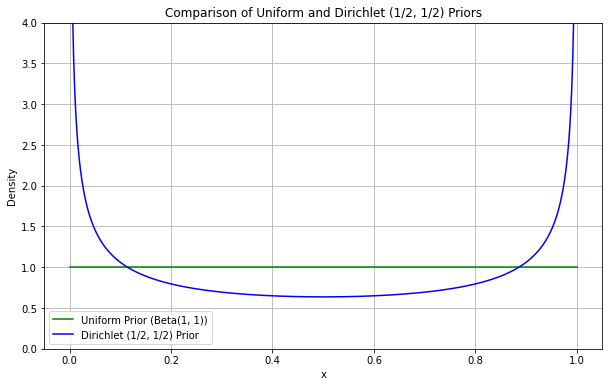
\includegraphics[height=6cm]{figures/dirichlet.png}
\end{frame}


\begin{frame}{Lemma 2: The $\mu$-Weighted Universal Portfolio}
    For the $\mu$-weighted universal portfolio:
    \R{\[
        \frac{S_n^*(x^n)}{\hat{S}_n(x^n)} 
        \leq \max\limits_{j^n} \frac{\prod\limits_{i=1}^{n} b^*_{j_i}}{\int_{\mathcal{B}} \prod\limits_{i=1}^{n} b_{j_i} \, d\mu(b)}
    \]}
    
    where the maximum is over the set of sequences of indices 
    \R{\[
        j^n \in \{1, \dots, m\}^n,
    \]}
    and 
    \R{\[
        \mathbf{b}^* = (b^*_1, \dots, b^*_m)^t
    \]}
    is the best constant rebalanced portfolio for the sequence \( x^n \).
\end{frame}

\begin{frame}
  \frametitle{Proof of Theorems}

  By Upper bounding
  \R{\[
      \max\limits_{j^n} \frac{\prod\limits_{i=1}^{n} b^*_{j_i}}{\int_{\mathcal{B}} \prod\limits_{i=1}^{n} b_{j_i} \, d\mu(b)}
    \]}
  For each prior distribution. 
\end{frame}


% Slide 1: Title Slide
\begin{frame}
    \centering
    \Huge Proof of Lemma 2
\end{frame}

% Slide 2: Recall the Definitions
\begin{frame}{Recall the Definitions}
    First, recall the definitions:
    \[
        S_n^*(x^n) = \prod_{i=1}^{n} b^{*t} x_i
    \]
    and
    \[
        \hat{S}_n(x^n) = \int_{\mathcal{B}} \prod_{i=1}^{n} b^t x_i \, d\mu(b).
    \]
\end{frame}

% Slide 3: Rewrite S_n^*(x^n)
\begin{frame}{Rewriting \( S_n^*(x^n) \)}
    We rewrite the product of sums \( S_n^*(x^n) \) as a sum of products.
    \[
        S_n^*(x^n) = \prod_{i=1}^{n} b^{*t} x_i
        = \prod_{i=1}^{n} \left( \sum_{j=1}^{m} b_j^* x_{ij} \right)
        = \sum_{j^n \in \{1, \dots, m\}^n} \prod_{i=1}^{n} b^*_{j_i} x_{j_i}
    \]
    Where
    \[
        j^n = (j_1, j_2, \dots, j_n) \in \{1, \dots, m\}^n.
    \]
\end{frame}

% Slide 5: Rewrite S_n(x^n)
\begin{frame}{Rewriting \( \hat{S}_n(x^n) \)}
    Similarly, we rewrite \( \hat{S}_n(x^n) \) as:
    \[
        \hat{S}_n(x^n) = \int_{\mathcal{B}} \prod_{i=1}^{n} b^t x_i \, d\mu(b)
    \]
    \[
        = \sum_{j^n \in \{1, \dots, m\}^n} \int_{\mathcal{B}} \prod_{i=1}^{n} b_{j_i} x_{ij_i} \, d\mu(b).
    \]
\end{frame}

% Slide 6: Ratio of Wealths
\begin{frame}{Ratio of Wealths}
    The ratio of wealths can now be written as:
    \[
        \frac{S_n^*(x^n)}{\hat{S}_n(x^n)}
        = \frac{\sum\limits_{j^n \in \{1, \dots, m\}^n} \prod\limits_{i=1}^{n} b^*_{j_i} x_{j_i}}
        {\sum\limits_{j^n \in \{1, \dots, m\}^n} \int_{\mathcal{B}} \prod\limits_{i=1}^{n} b_{j_i} x_{ij_i} \, d\mu(b)}
    \]
\end{frame}

% Slide 7: Alternative Formulation of Ratio
\begin{frame}{Alternative Formulation of Ratio}
    \[
        \frac{S_n^*(x^n)}{\hat{S}_n(x^n)}
        = \frac{\sum\limits_{j^n: \prod\limits_{i=1}^{n} x_{ij_i} > 0} \prod\limits_{i=1}^{n} b^*_{j_i} x_{j_i}}
        {\sum\limits_{j^n: \prod\limits_{i=1}^{n} x_{ij_i} > 0} \int_{\mathcal{B}} \prod\limits_{i=1}^{n} b_{j_i} x_{ij_i} \, d\mu(b)}
    \]
\end{frame}

\begin{frame}{Lemma 1}
    If $\alpha_1, \dots, \alpha_n \geq 0$, and $\beta_1, \dots, \beta_n \geq 0$, then
    \[
        \frac{\sum\limits_{i=1}^{n} \alpha_i}{\sum\limits_{i=1}^{n} \beta_i} 
        \leq \max\limits_{j} \frac{\alpha_j}{\beta_j}.
    \]
\end{frame}


% Slide 1: Applying Lemma 1
\begin{frame}{Applying Lemma 1}
    We apply Lemma 1 with:
    \[
        \alpha_{(j^n)} \triangleq \prod_{i=1}^{n} b^*_{j_i} x_{ij_i}
    \]
    and
    \[
        \beta_{(j^n)} \triangleq \int_{\mathcal{B}} \prod_{i=1}^{n} b_{j_i} x_{ij_i} \, d\mu(b)
    \]
    for
    \[
        j^n \in \left\{ j^n: \prod_{i=1}^{n} x_{ij_i} > 0 \right\}.
    \]
\end{frame}

% Slide 2: Obtaining the Bound
\begin{frame}{Obtaining the Bound}
    Using Lemma 1, we obtain:
    \[
        \frac{S_n^*(x^n)}{\hat{S}_n(x^n)}
        \leq \max\limits_{j^n: \prod\limits_{i=1}^{n} x_{ij_i} > 0}
        \frac{\prod\limits_{i=1}^{n} b^*_{j_i} x_{ij_i}}
        {\int_{\mathcal{B}} \prod\limits_{i=1}^{n} b_{j_i} x_{ij_i} \, d\mu(b)}
    \]
\end{frame}

% Slide 3: Simplifying the Expression
\begin{frame}{Simplifying the Expression}
    The fraction simplifies to:
    \[
        = \max\limits_{j^n: \prod\limits_{i=1}^{n} x_{ij_i} > 0}
        \frac{\prod\limits_{i=1}^{n} b^*_{j_i}}
        {\int_{\mathcal{B}} \prod\limits_{i=1}^{n} b_{j_i} \, d\mu(b)}
    \]
    \[
        \leq \max\limits_{j^n} \frac{\prod\limits_{i=1}^{n} b^*_{j_i}}
        {\int_{\mathcal{B}} \prod\limits_{i=1}^{n} b_{j_i} \, d\mu(b)}
    \]
\end{frame}

% Slide 4: Completing the Proof
\begin{frame}{Completing the Proof}
    Since the product of \( x_{ij_i} \)'s factors out of the numerator and denominator, we conclude:
    \[
        \frac{S_n^*(x^n)}{\hat{S}_n(x^n)}
        \leq \max\limits_{j^n} \frac{\prod\limits_{i=1}^{n} b^*_{j_i}}
        {\int_{\mathcal{B}} \prod\limits_{i=1}^{n} b_{j_i} \, d\mu(b)}
    \]
\end{frame}

\begin{frame}{Some real-world examples.}
    \begin{itemize}
    \item 2-stock portfolios
    \item Period:1963 - 1985
    \item Kin Arc and Iroquis are two of the most volatile stocks.
    \item Iroquis was the best performing stock for this period (791\% profit)
    \end{itemize}
\end{frame}


% Slide 4
\begin{frame}
\frametitle{Iroqu vs. Kinar}
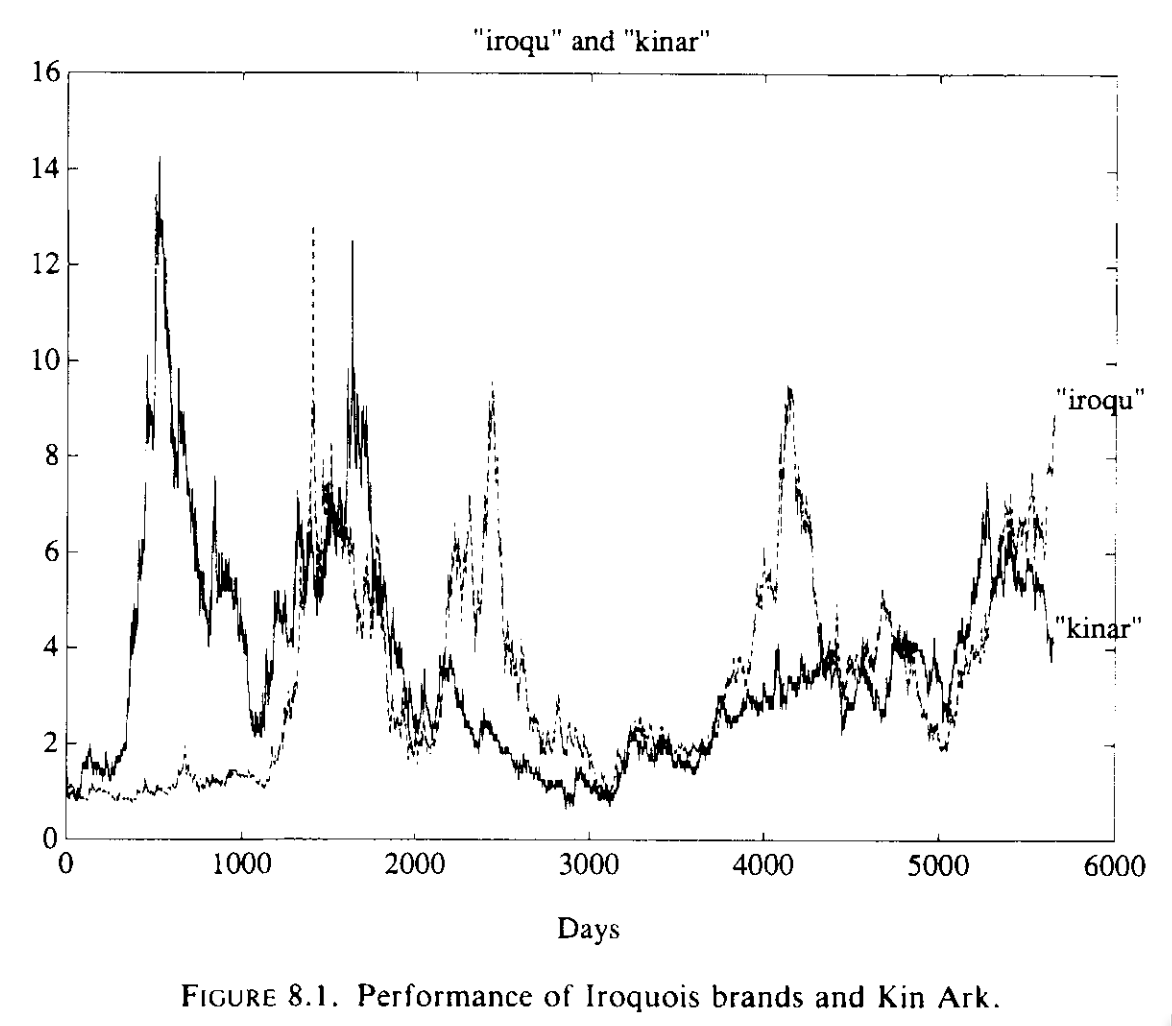
\includegraphics[height=7cm]{figures/Cursor_and_Universal_Portfolios_pdf-3.png}
\end{frame}

% Slide 3
\begin{frame}
\frametitle{Iroqu vs. Kinar vs Universal}
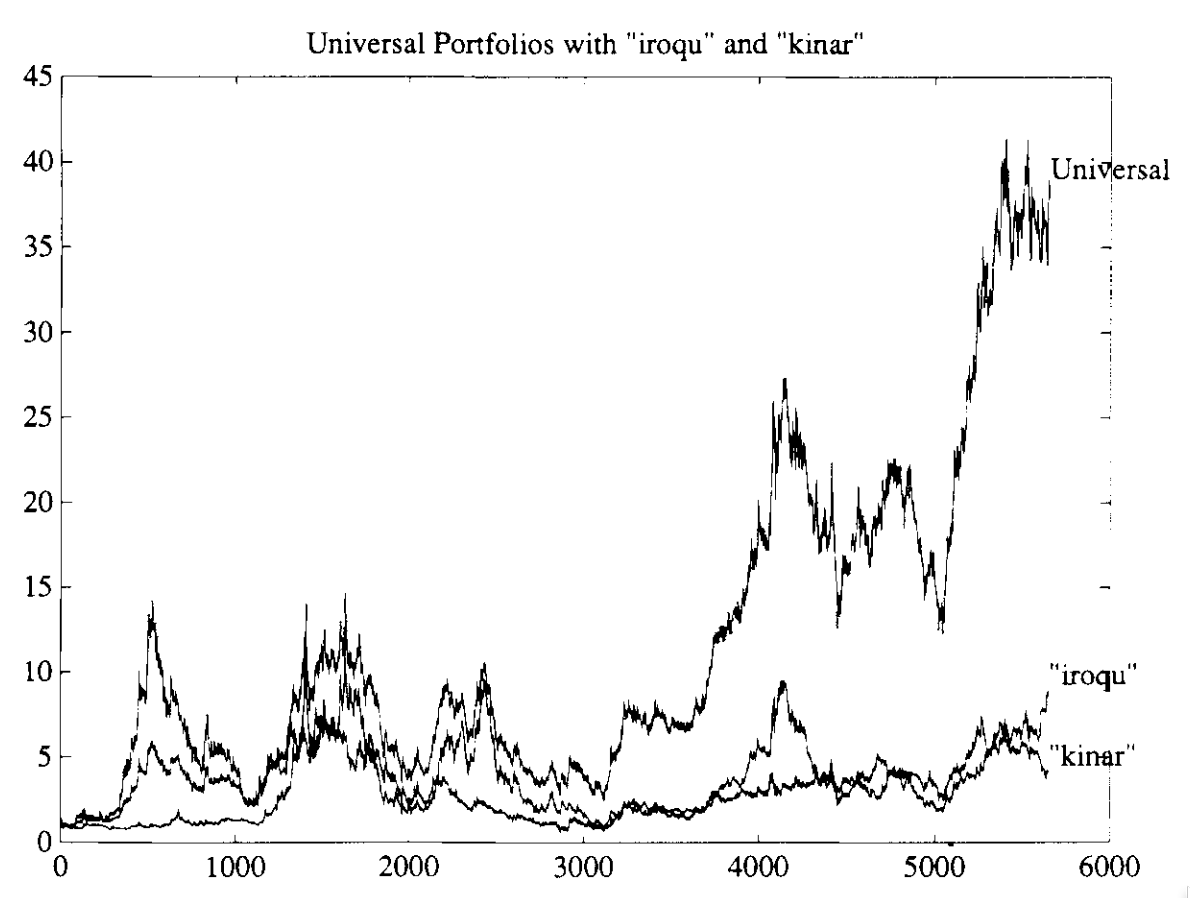
\includegraphics[height=7cm]{figures/Cursor_and_Universal_Portfolios_pdf-2.png}
\end{frame}

% Slide 5
\begin{frame}
\frametitle{Iroqu vs. Kinar 20yr return of different fixed portfolios}

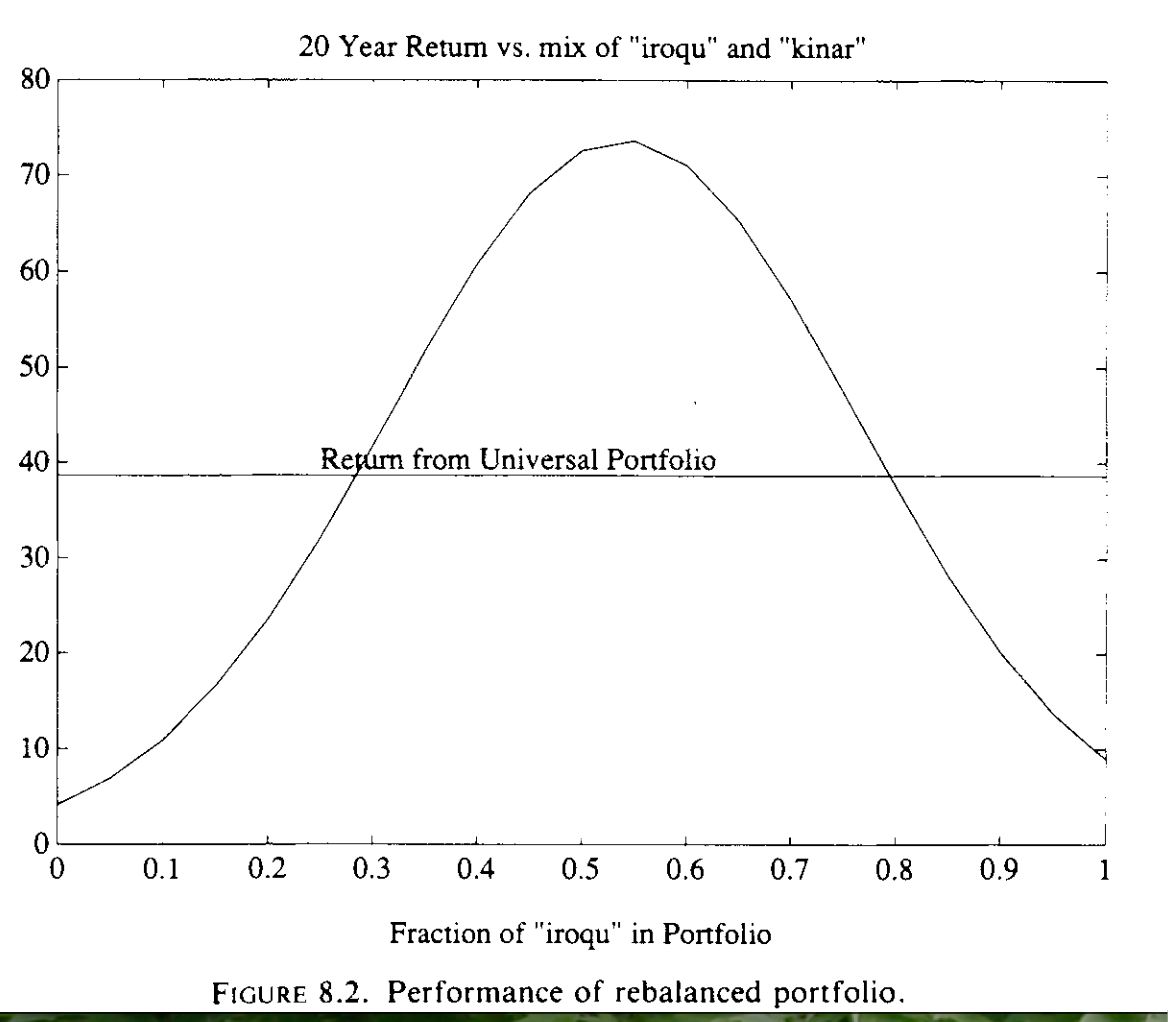
\includegraphics[height=7cm]{figures/Cursor_and_Universal_Portfolios_pdf-4.png}
\end{frame}

% Slide 6
\begin{frame}
\frametitle{Iroqu vs. Kinar mix in universal portfolio}

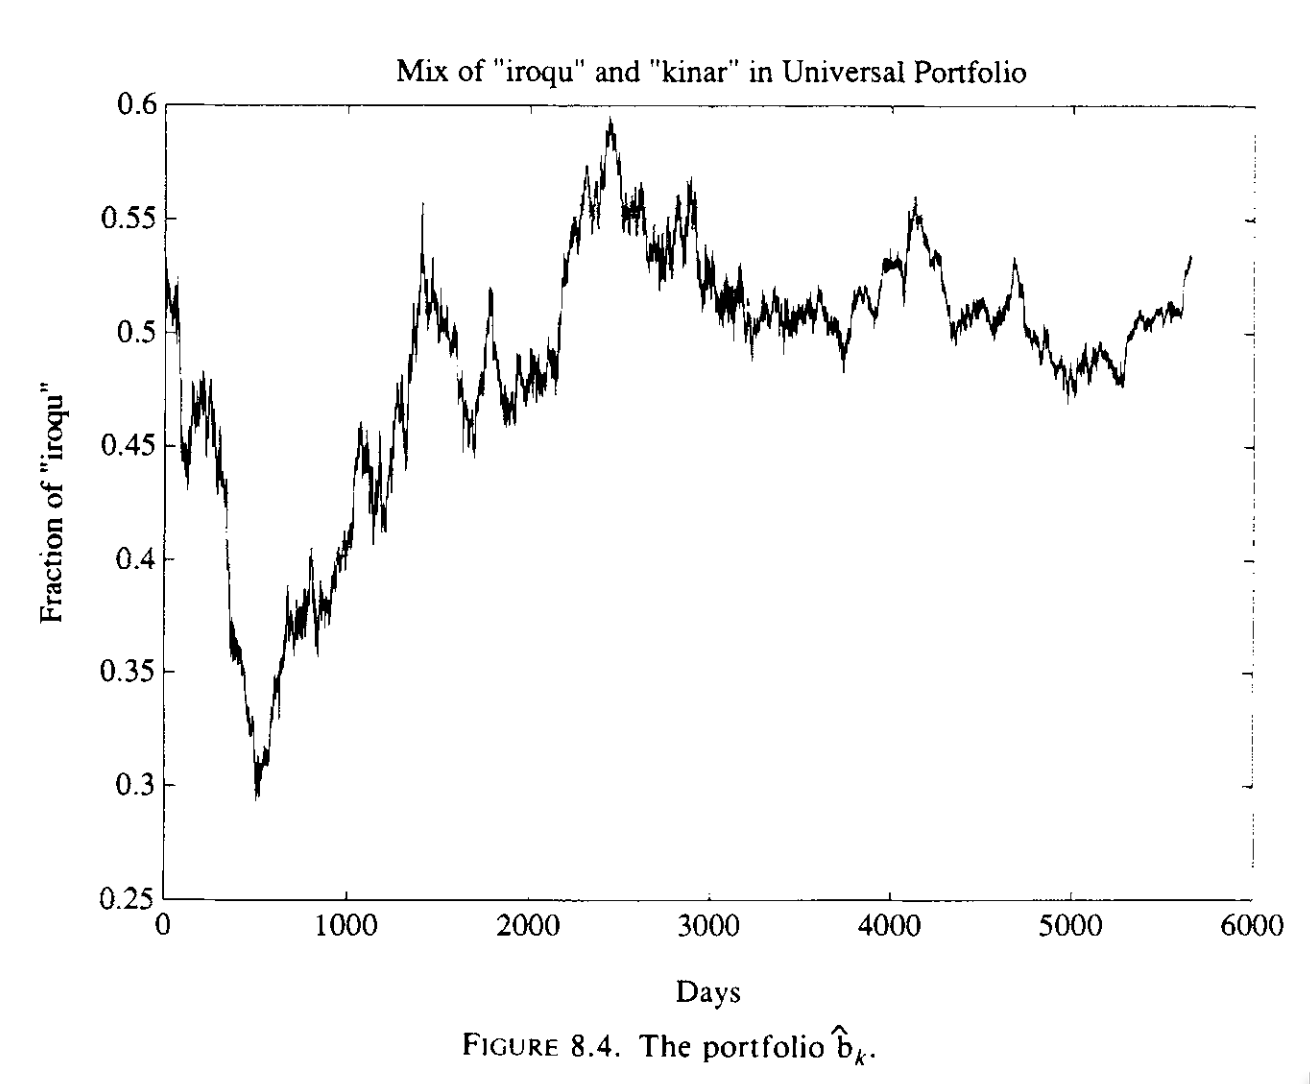
\includegraphics[height=7cm]{figures/Cursor_and_Universal_Portfolios_pdf.png}
\end{frame}

% Slide 1
\begin{frame}
\frametitle{Commercial Metals and Kin Arc}
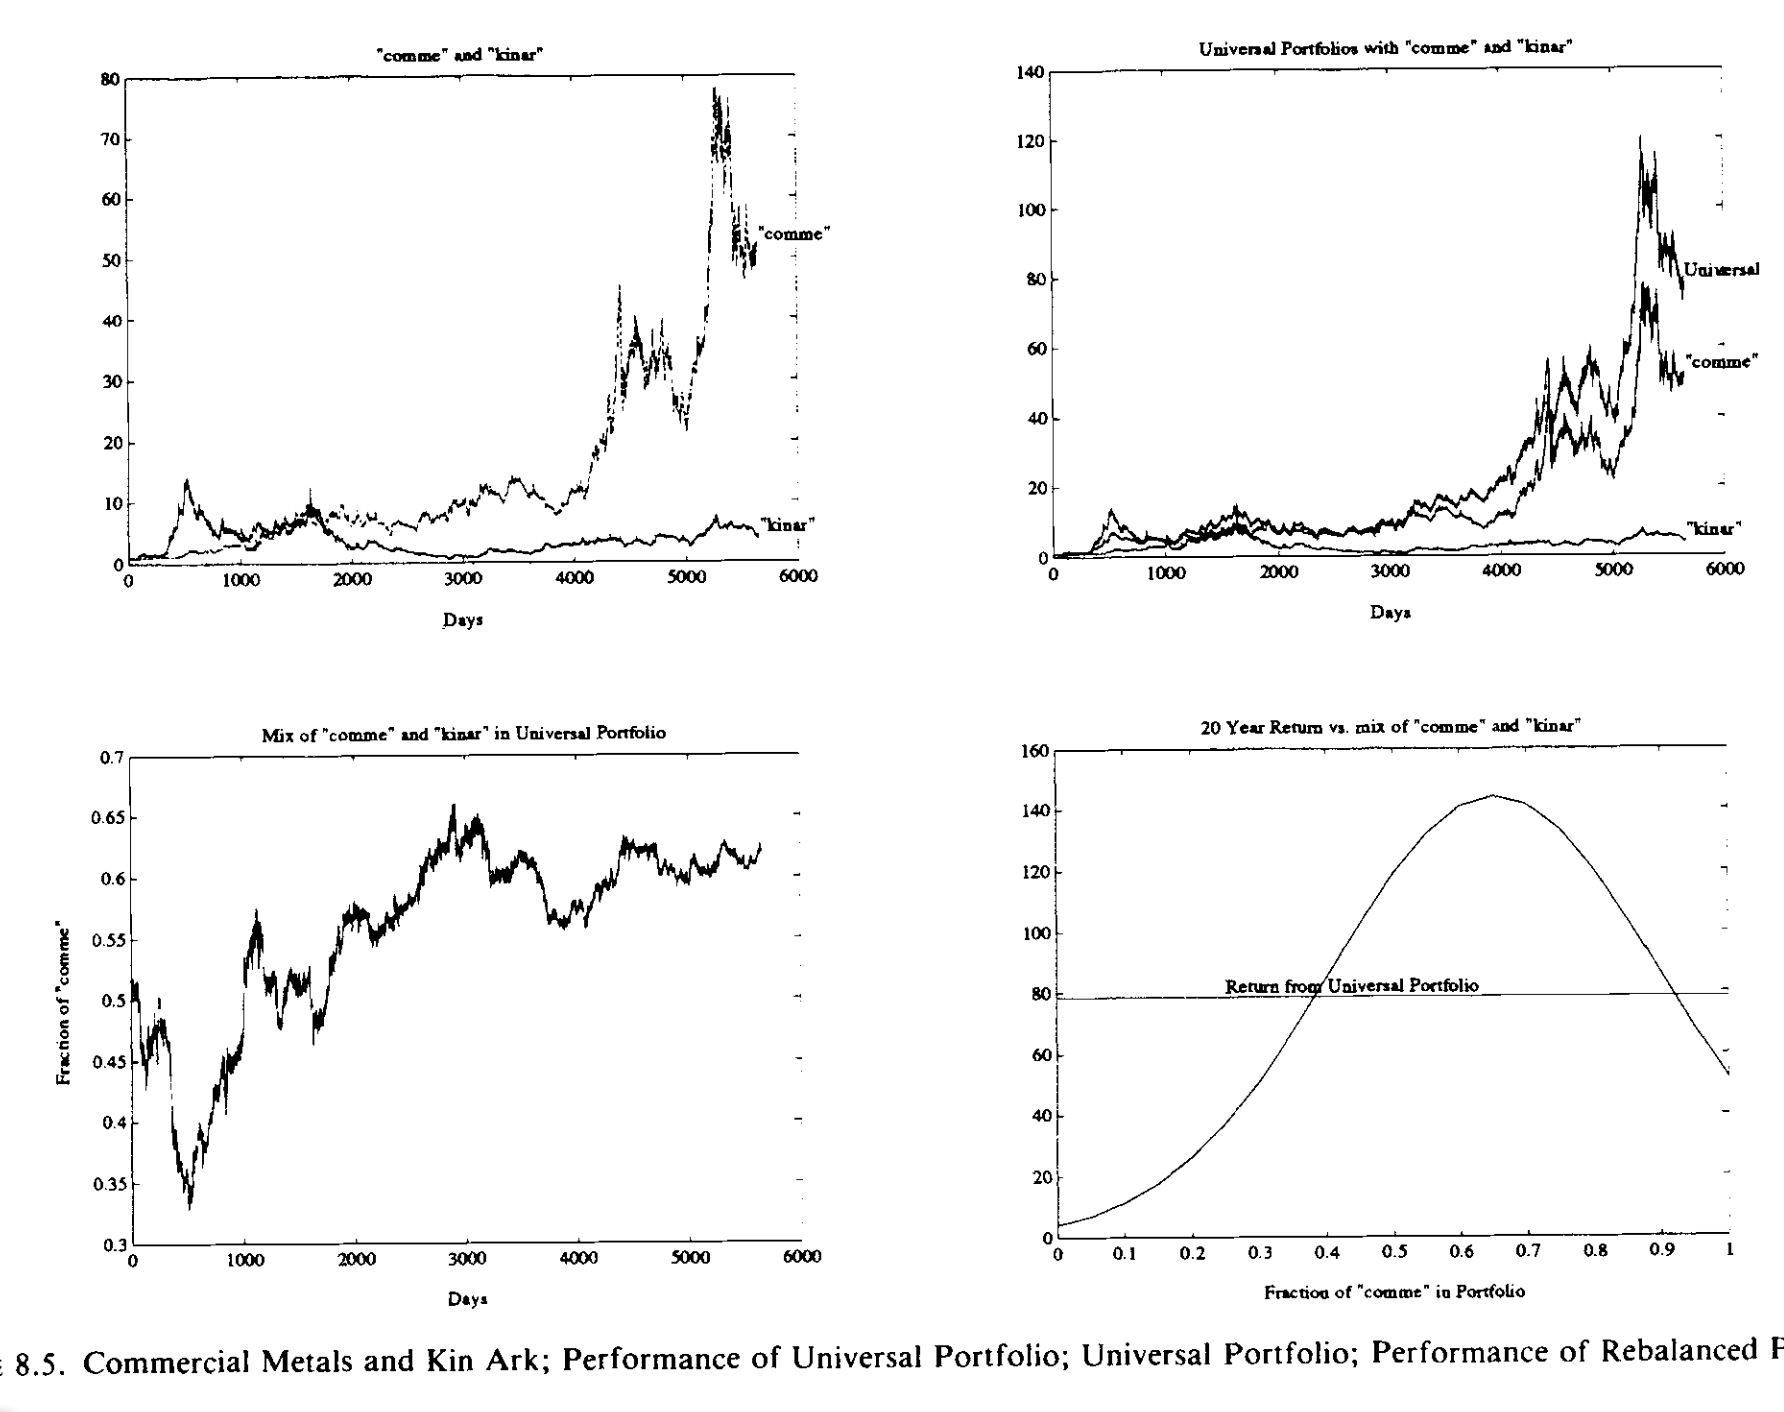
\includegraphics[height=7cm]{figures/CommercialMetals&KinArc.png}
\end{frame}

% Slide 2
\begin{frame}
\frametitle{Commercial Metals and Mei Corp}
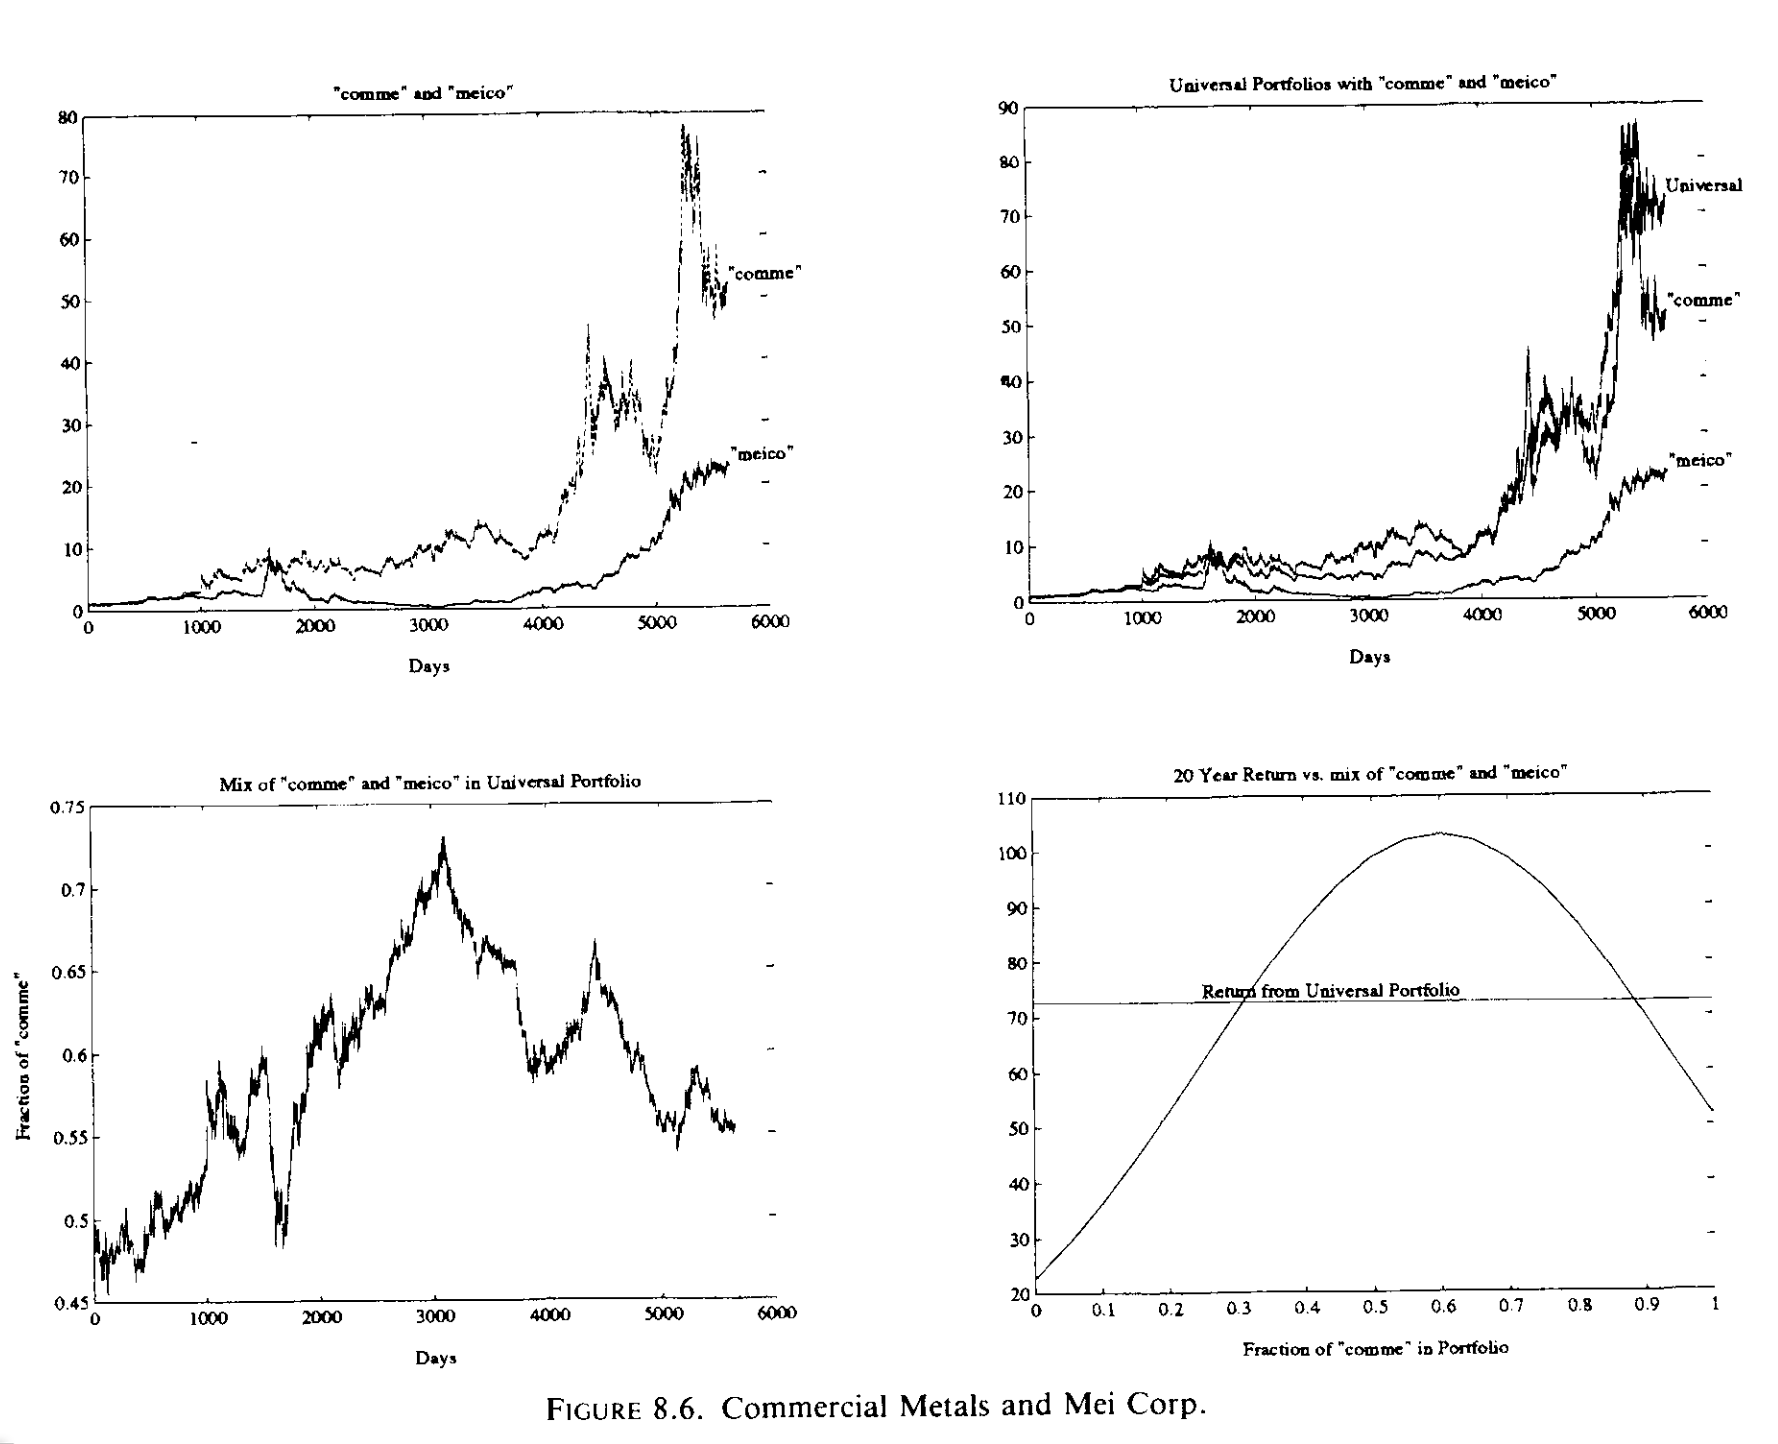
\includegraphics[height=7cm]{figures/CommercialMetals&MeiCorp.png}
\end{frame}

% Slide 7
\begin{frame}
\frametitle{IBM and CocaCola}
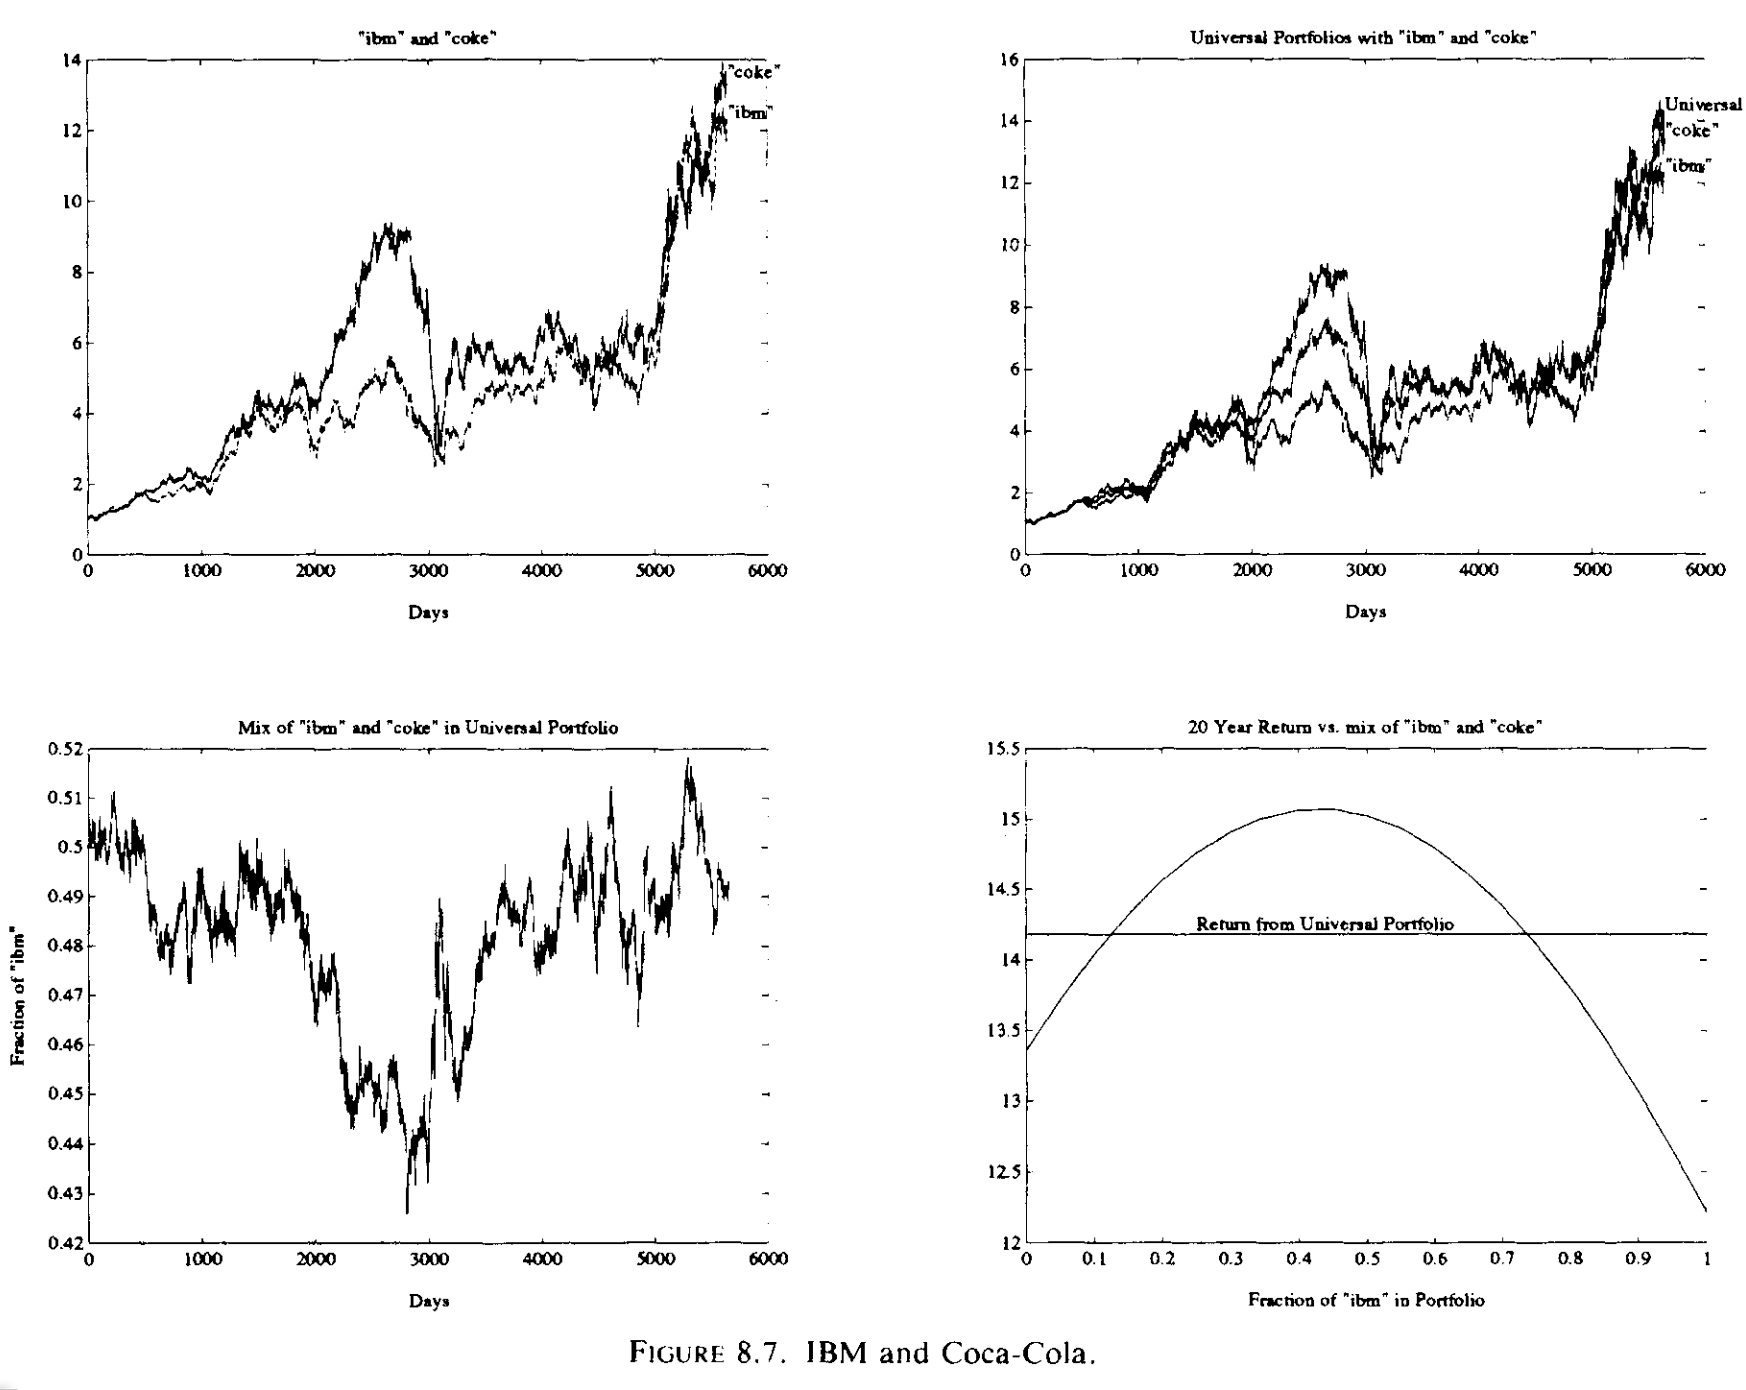
\includegraphics[height=7cm]{figures/IBM&CocaCola.png}
\end{frame}

\begin{frame}
  \frametitle{Some issues}
  \begin{itemize}
  \item Transaction costs are ignored.
  \item Stocks selected in hind-sight.
  \item Volatile stocks are sensitive to exit time.
  \item Ignores mergers bankruptcies and acquisitions.
  \end{itemize}
\end{frame}

\iffalse
%------------------------------------------------
\section{Basic Setup}
%------------------------------------------------
\begin{frame}{Model Setup}
  \begin{itemize}
    \item Consider a market with \(m\) assets (e.g.\ stocks).
    \item Trading occurs in \(\textbf{discrete time}\): \(t = 1, 2, \ldots, n\).
    \item Let \(x_{t} \in \mathbb{R}^m\) be the gross returns of the \(m\) assets between time \(t-1\) and \(t\).
      \begin{itemize}
        \item For example, if the \(j\)-th asset goes up by \(2\%\), then \(x_{t}^{(j)} = 1.02\).
      \end{itemize}
    \item A portfolio vector \(b_t \in \mathbb{R}^m\) specifies how one’s capital is allocated among the \(m\) assets at time \(t\).
      \begin{itemize}
        \item The entries of \(b_t\) sum to 1 and are nonnegative: \(\sum_{j=1}^m b_t^{(j)} = 1\), \(b_t^{(j)} \ge 0\).
      \end{itemize}
  \end{itemize}
\end{frame}

%------------------------------------------------
\begin{frame}{Wealth Evolution}
  \begin{itemize}
    \item Let \(S_t\) denote the wealth at time \(t\).
    \item Given a portfolio \(b_t\) at time \(t\), the wealth is updated by
      \[
        S_{t+1} = S_t \, \bigl( b_t \cdot x_{t+1} \bigr),
      \]
      where \(b_t \cdot x_{t+1}\) is the dot product of \(b_t\) and \(x_{t+1}\).
    \item The goal is to choose \(\{b_t\}_{t=1}^n\) to maximize the final wealth \(S_{n+1}\) or equivalently 
          \(\log S_{n+1}\).
  \end{itemize}
\end{frame}

%------------------------------------------------
\section{Definition of the Universal Portfolio}
%------------------------------------------------
\begin{frame}{Cover's Universal Portfolio (Informal Definition)}
  \begin{enumerate}
    \item \textbf{Consider all constant-rebalanced portfolios.} A constant-rebalanced portfolio (CRP) 
          is one that keeps the same fraction in each asset at every time step.
    \item \textbf{Assign a prior.} Treat each CRP as an element in the simplex of possible weights \(b \in \Delta^m\). 
          Typically, one uses the \emph{Dirichlet} (or uniform) prior over the simplex.
    \item \textbf{Update posterior.} After each period, update this distribution (the mixture) over all CRPs 
          based on how well each CRP performed.
    \item \textbf{Form the next investment by averaging.} Allocate the portfolio \(b_{t+1}\) as a weighted average 
          of all possible CRPs, weighted by their posterior performance.
  \end{enumerate}
  \[
    b_{t+1} = \int b \, d\mu_t(b),
  \]
  where \(\mu_t\) is the posterior over the simplex after observing \(t\) periods.
\end{frame}

%------------------------------------------------
\begin{frame}{Key Result}
  \begin{itemize}
    \item \textbf{Asymptotic Optimality:} Cover showed that the growth rate of the \emph{universal portfolio} 
          will, in the limit, approach the growth rate of the best \emph{single} constant-rebalanced portfolio 
          in hindsight.
    \item Formally, let \(b^*\) be the CRP that maximizes \(\log S_n\) in hindsight. Then the ratio of 
          the universal portfolios wealth \(U_n\) to the wealth of \(b^*\) (both starting at 1) 
          grows sub-exponentially in \(n\). 
    \[
      \frac{U_n}{S_n(b^*)} \ge \exp(-o(n)) \quad \text{as } n \to \infty.
    \]
    \item This means that the universal portfolio is \emph{universally} good, without prior knowledge 
          of which CRP is best.
  \end{itemize}
\end{frame}

%------------------------------------------------
\section{Implementation Details}
%------------------------------------------------
\begin{frame}{Practical Construction}
  \begin{enumerate}
    \item \textbf{Discretize the Simplex:}
      \begin{itemize}
        \item In practice, the integral over all \(b\) in the simplex is approximated by a finite grid or sampling.
      \end{itemize}
    \item \textbf{Recompute Weights:}
      \[
        w_{t+1}(b) = \frac{w_t(b)\cdot \bigl(b \cdot x_{t+1}\bigr)}{\int w_t(u)\cdot \bigl(u \cdot x_{t+1}\bigr)\,du}
      \]
      where \(w_t(b)\) is the weight or a-posteriori for CRP \(b\).
    \item \textbf{Compute New Investment:}
      \[
        b_{t+1} = \int b \, w_{t+1}(b)\,db \quad \approx \sum_{b \in \mathcal{B}} b \, w_{t+1}(b).
      \]
    \item \textbf{Rebalance Accordingly:} Actually execute \(b_{t+1}\) in the market at time \(t+1\).
  \end{enumerate}
\end{frame}

%------------------------------------------------
\section{Example}
%------------------------------------------------
\begin{frame}{Simple Example (2 Assets)}
  \begin{itemize}
    \item Suppose there are 2 assets, so \(b \in [0,1]\) with \(b_1 = b\), \(b_2 = 1-b\).
    \item \textbf{Uniform Prior:} Start with \(w_0(b) = 1\) for \(b \in [0,1]\).
    \item \textbf{Observations:} If the asset returns over first period are \((x_1, x_2)\), then after seeing 
          that outcome, the weight function updates:
      \[
        w_1(b) \propto b \, x_1 + (1-b) \, x_2.
      \]
    \item \textbf{Next Step:} The universal strategy at \(t=1\) invests
      \[
        b_1 = \int_0^1 b \,\frac{b \, x_1 + (1-b) \, x_2}{Z} \, db,
      \]
      where \(Z\) is a normalization constant to ensure the posterior integrates to 1.
  \end{itemize}
\end{frame}

%------------------------------------------------
\begin{frame}{Numerical Illustration}
  \begin{itemize}
    \item By discretizing \(b \in [0,1]\) into many small steps, you can numerically approximate the integrals.
    \item Over time, the algorithm will put more weight on the best fraction \(b^*\) that maximizes growth, 
          but it still accounts for uncertainty and adapts as the environment changes.
  \end{itemize}
\end{frame}

%------------------------------------------------
\section{Summary and References}
%------------------------------------------------
\begin{frame}{Summary}
  \begin{itemize}
    \item \textbf{Cover's Universal Portfolio} is a powerful idea that uses mixture methods over all possible 
          constant-rebalanced portfolios.
    \item \textbf{Guarantees:} It asymptotically matches the best constant-rebalanced strategy in hindsight.
    \item \textbf{Implementation:} Although conceptually elegant, the naive integral approach can be computationally 
          expensive. Practical approximations are used (discretization, sampling, etc.).
    \item \textbf{Significance:} This method bridges information theory and portfolio choice, 
          illustrating how universal strategies can learn from the market without predictions.
  \end{itemize}
\end{frame}
\fi

\end{small}


\end{document}

%%% Local Variables:
%%% mode: latex
%%% TeX-master: t
%%% End:
